%
% radonft.tex -- radon transform and fourier transform
%
% (c) 2021 Prof Dr Andreas Müller, OST Ostschweizer Fachhochschule
%
\documentclass[tikz]{standalone}
\usepackage{amsmath}
\usepackage{times}
\usepackage{txfonts}
\usepackage{pgfplots}
\usepackage{csvsimple}
\usepackage{mathrsfs}
\usetikzlibrary{arrows,intersections,math}
\begin{document}
\def\skala{1}
\def\w{65}
\def\r{2.2}
\pgfmathparse{6*\w/180-3}
\definecolor{darkgreen}{rgb}{0,0.8,0}
\definecolor{polarcolor}{rgb}{1,0,0}
\definecolor{pointcolor}{rgb}{0,1,1}
\xdef\wh{\pgfmathresult}
\begin{tikzpicture}[>=latex,thick,scale=\skala]
\clip (-3,3.7) rectangle (11,-11.1);

\node at (0,3) [above] {Ortsraum\strut};

\begin{scope}[xshift=7.6cm]
\fill[color=darkgreen!10] (-3.4,-11.1) rectangle (3.4,3.7);
\node[color=darkgreen] at (0,3) [above] {Wellenzahlebene\strut};
\end{scope}

\begin{scope}
	\clip (-3,-3) rectangle (3,3);
	\node at (0,0) [rotate=0] {
\includegraphics[width=6cm]{mathman.jpg}};
	\fill[color=polarcolor!10!white,opacity=0.7]
		(0,0) -- (1.5,0) arc (0:\w:1.5) -- cycle;
	\draw[color=polarcolor] (0,0) -- (1.5,0) arc (0:\w:1.5);
	\node[color=polarcolor] at ({\w/2}:1) {$\varphi$};
	\draw[color=polarcolor] ({\w+180}:5) -- ({\w}:5);
	\begin{scope}[rotate=\w]
	\foreach \d in {-5,-4.5,...,5}{
		\draw[line width=0.1pt,color=pointcolor] (\d,-5) -- (\d,5);
		\fill[color=pointcolor] (\d,0) circle[radius=0.03];
	}
	\end{scope}
\end{scope}

\begin{scope}[yshift=-7.6cm]
	\node at (0,0) {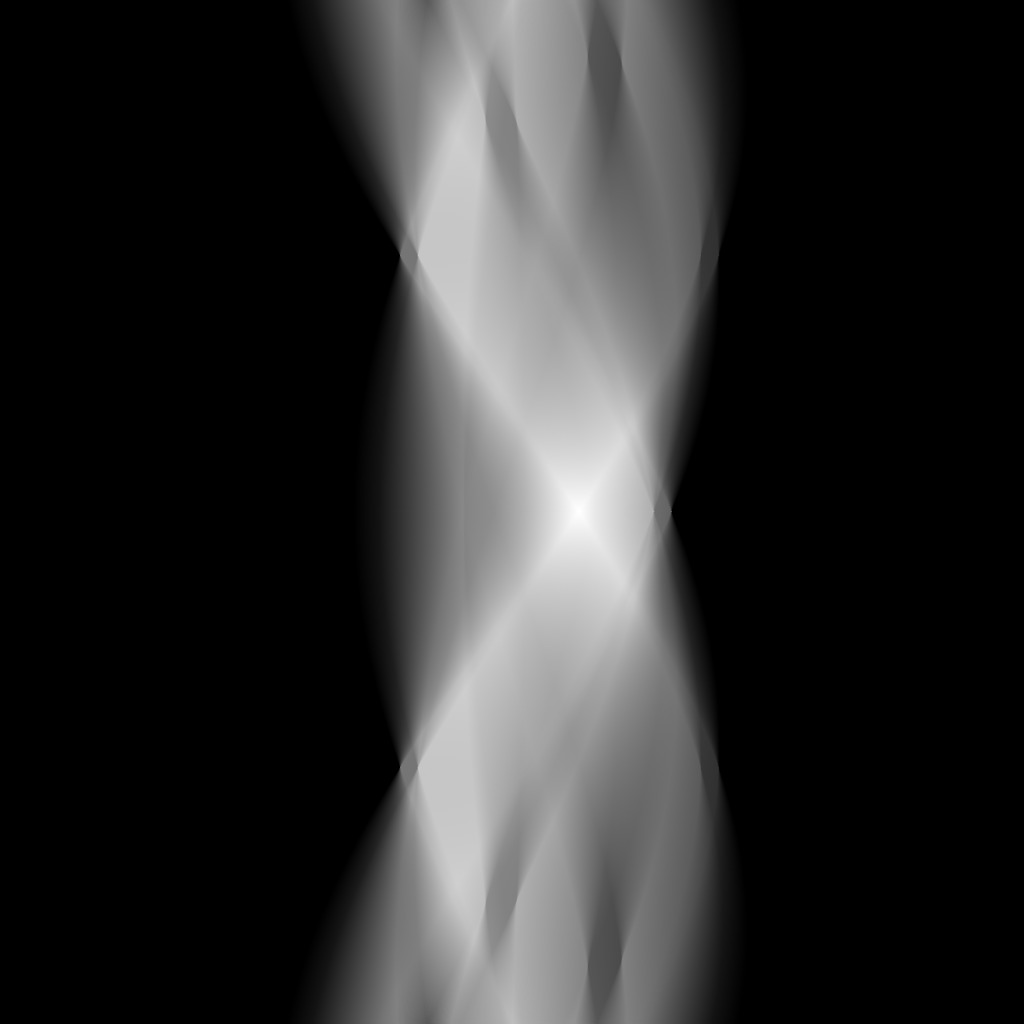
\includegraphics[width=6cm]{mathman-radon.jpg}};
	\draw[color=pointcolor] (-3,\wh) -- (3,\wh);
	\draw[->,color=polarcolor] (0,-3) -- (0,3.3)
		coordinate[label={right:$\varphi$}];
	\draw[->,color=polarcolor] (-3,-3) -- (3.2,-3) coordinate[label={$r$}];
	\fill[color=polarcolor] (0,-3) circle[radius=0.05];
	\foreach \y in {0,3}{
		\draw[color=polarcolor] (-0.05,\y) -- (0.05,\y);
	}
	\node[color=polarcolor] at (0,3) [below left] {$\scriptstyle \pi\mathstrut$};
	\node[color=polarcolor] at (0,0) [left] {$\frac{\pi}{2}\mathstrut$};
	\node[color=polarcolor] at (0,-3) [above left] {$\scriptstyle 0\mathstrut$};
\end{scope}

\begin{scope}[xshift=7.6cm,yshift=-7.6cm]
	\node at (0,0)
		{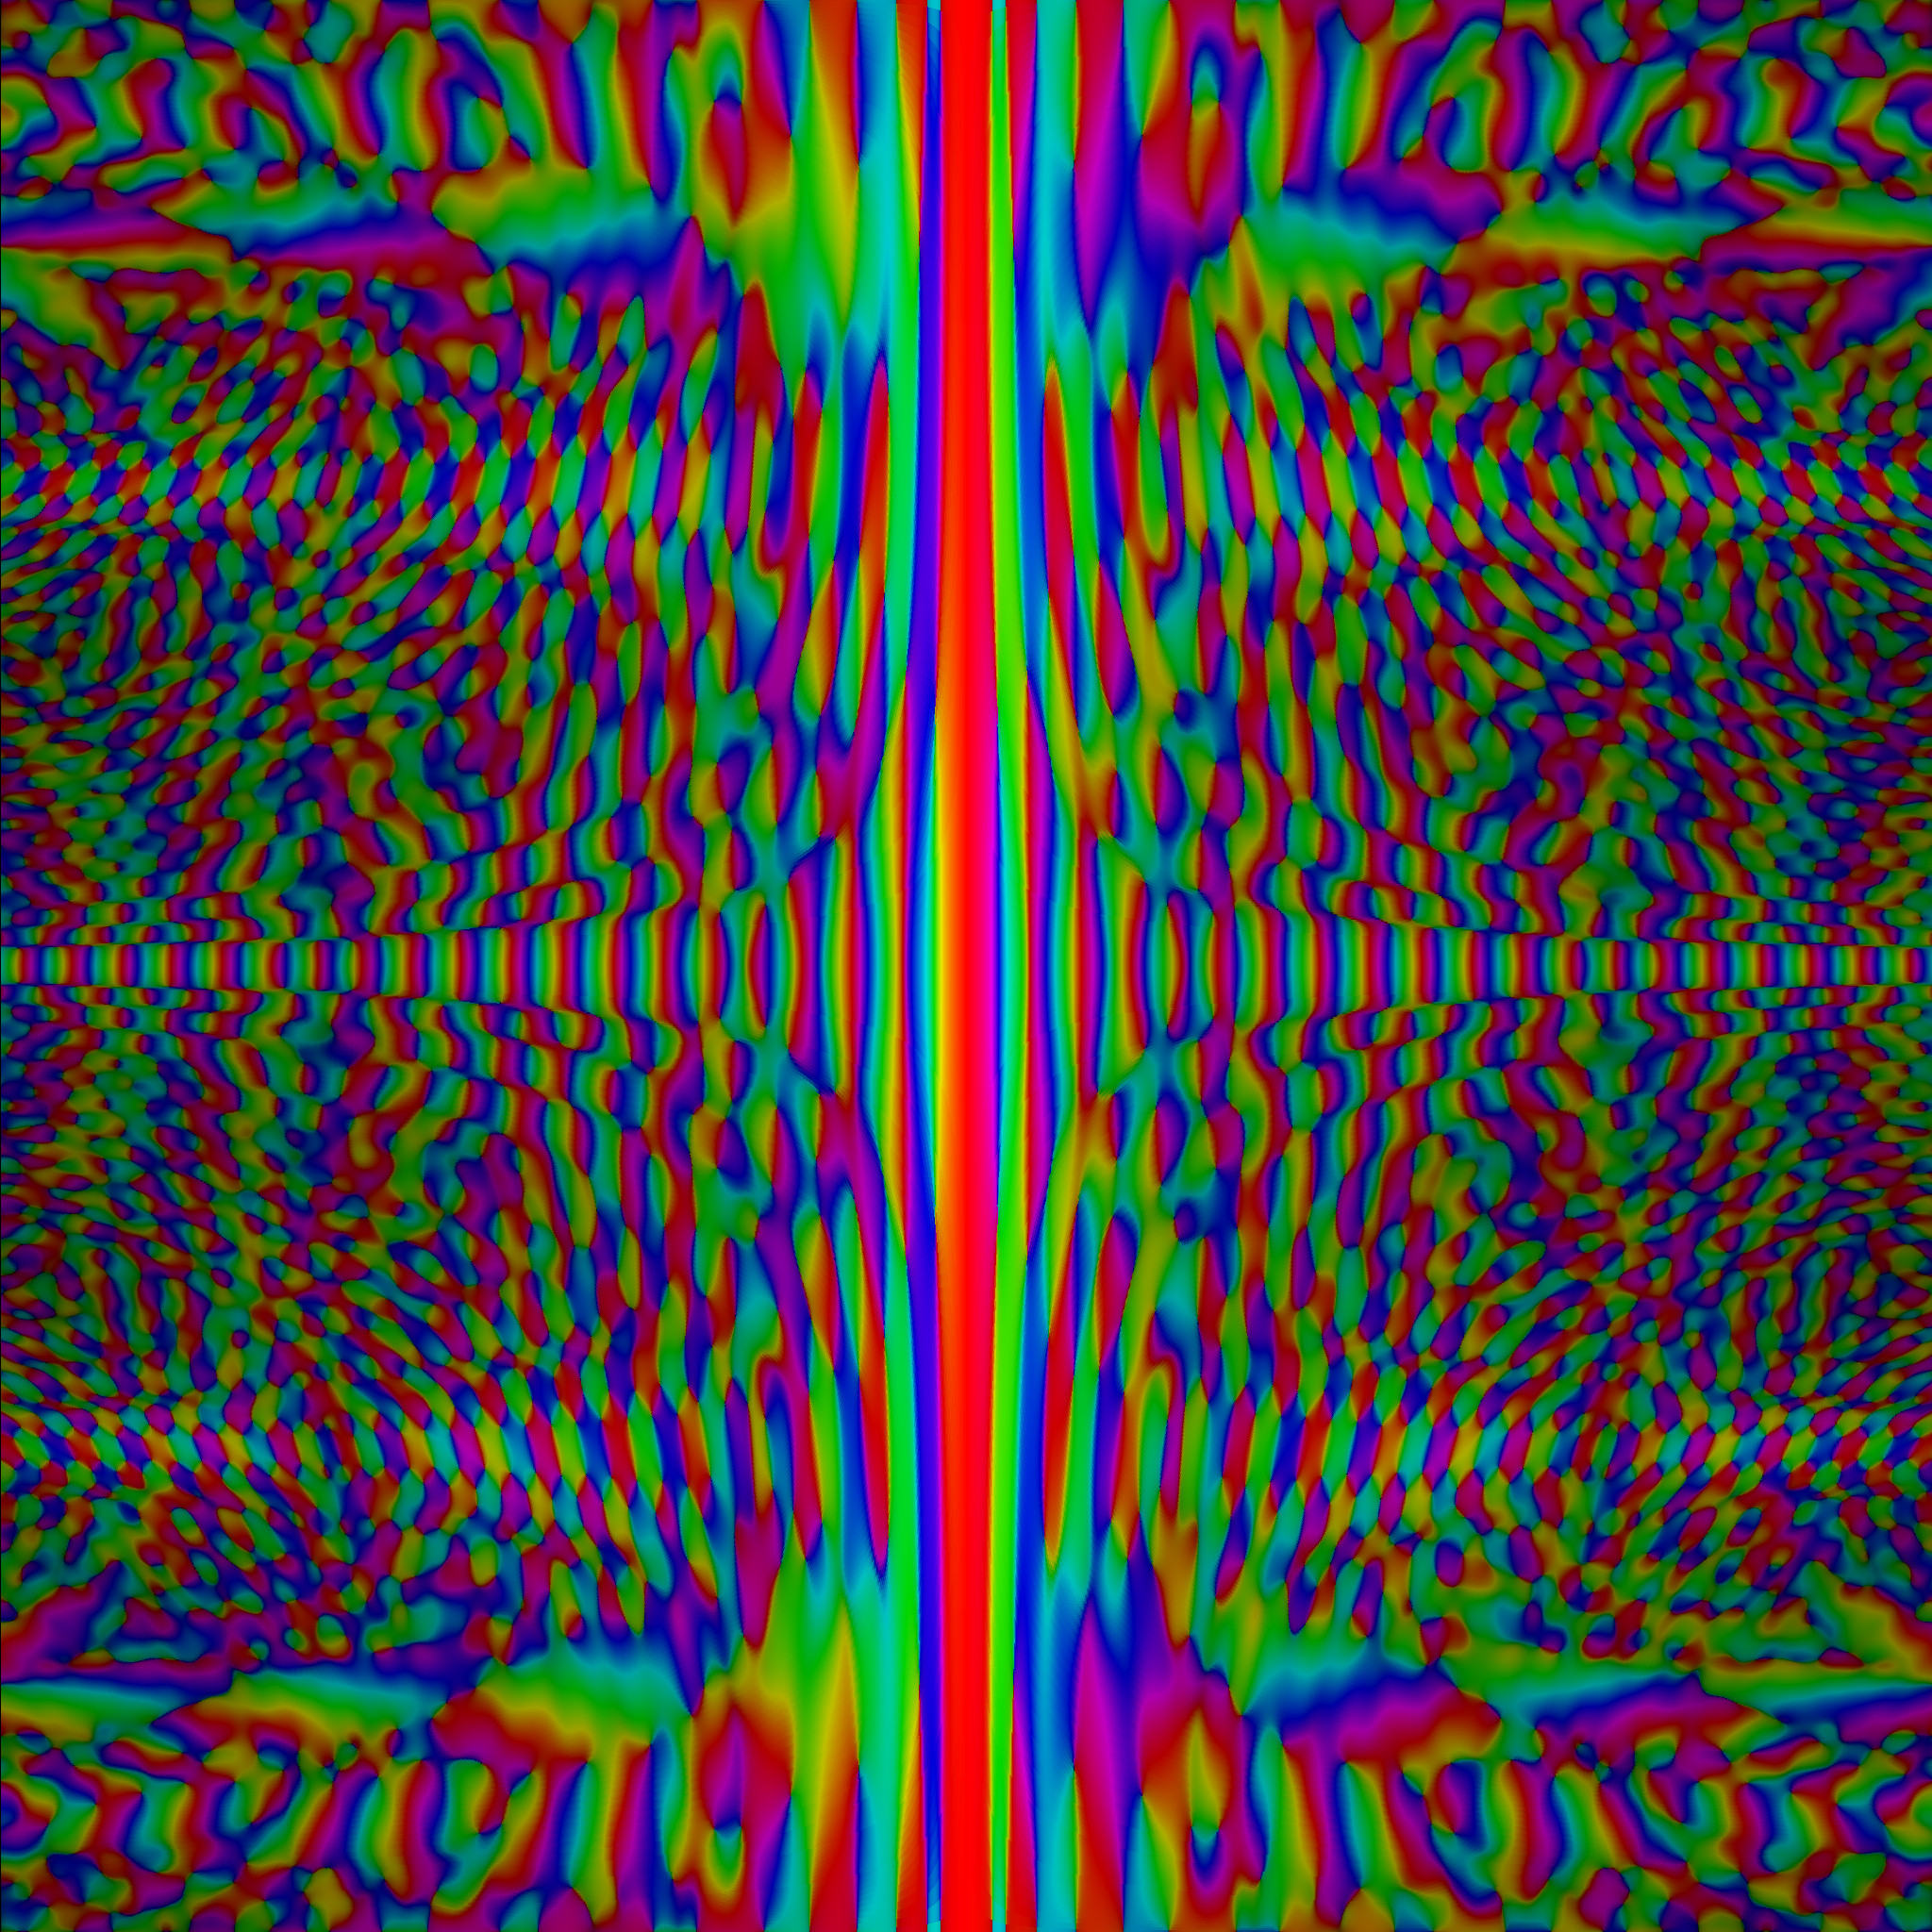
\includegraphics[width=6cm]{mathman2-backward-FT-polar.jpg}};
	\draw[->,color=polarcolor]
		(0,-3) -- (0,3.4) coordinate[label={right:$\varphi$}];
	\fill[color=polarcolor] (0,-3) circle[radius=0.05];
	\draw[color=white] (0,-3) -- (0,3);
	\node at (0,-3) [below] {$0$};
	\draw[->,color=polarcolor] (-3,-3) -- (3.3,-3) coordinate[label={$r$}];
	\draw[color=pointcolor] (-3,{\wh}) -- (3,{\wh});
	%\draw[color=pointcolor] (\r,-3) -- (\r,3);
	\fill[color=pointcolor] (\r,\wh) circle[radius=0.08];
	\node[color=pointcolor] at (\r,\wh) [above] {$(r,\varphi)$};
\end{scope}

\begin{scope}[xshift=7.6cm]
	\begin{scope}
	\clip (0,0) circle[radius=3cm];
	\node at (0,0)
	{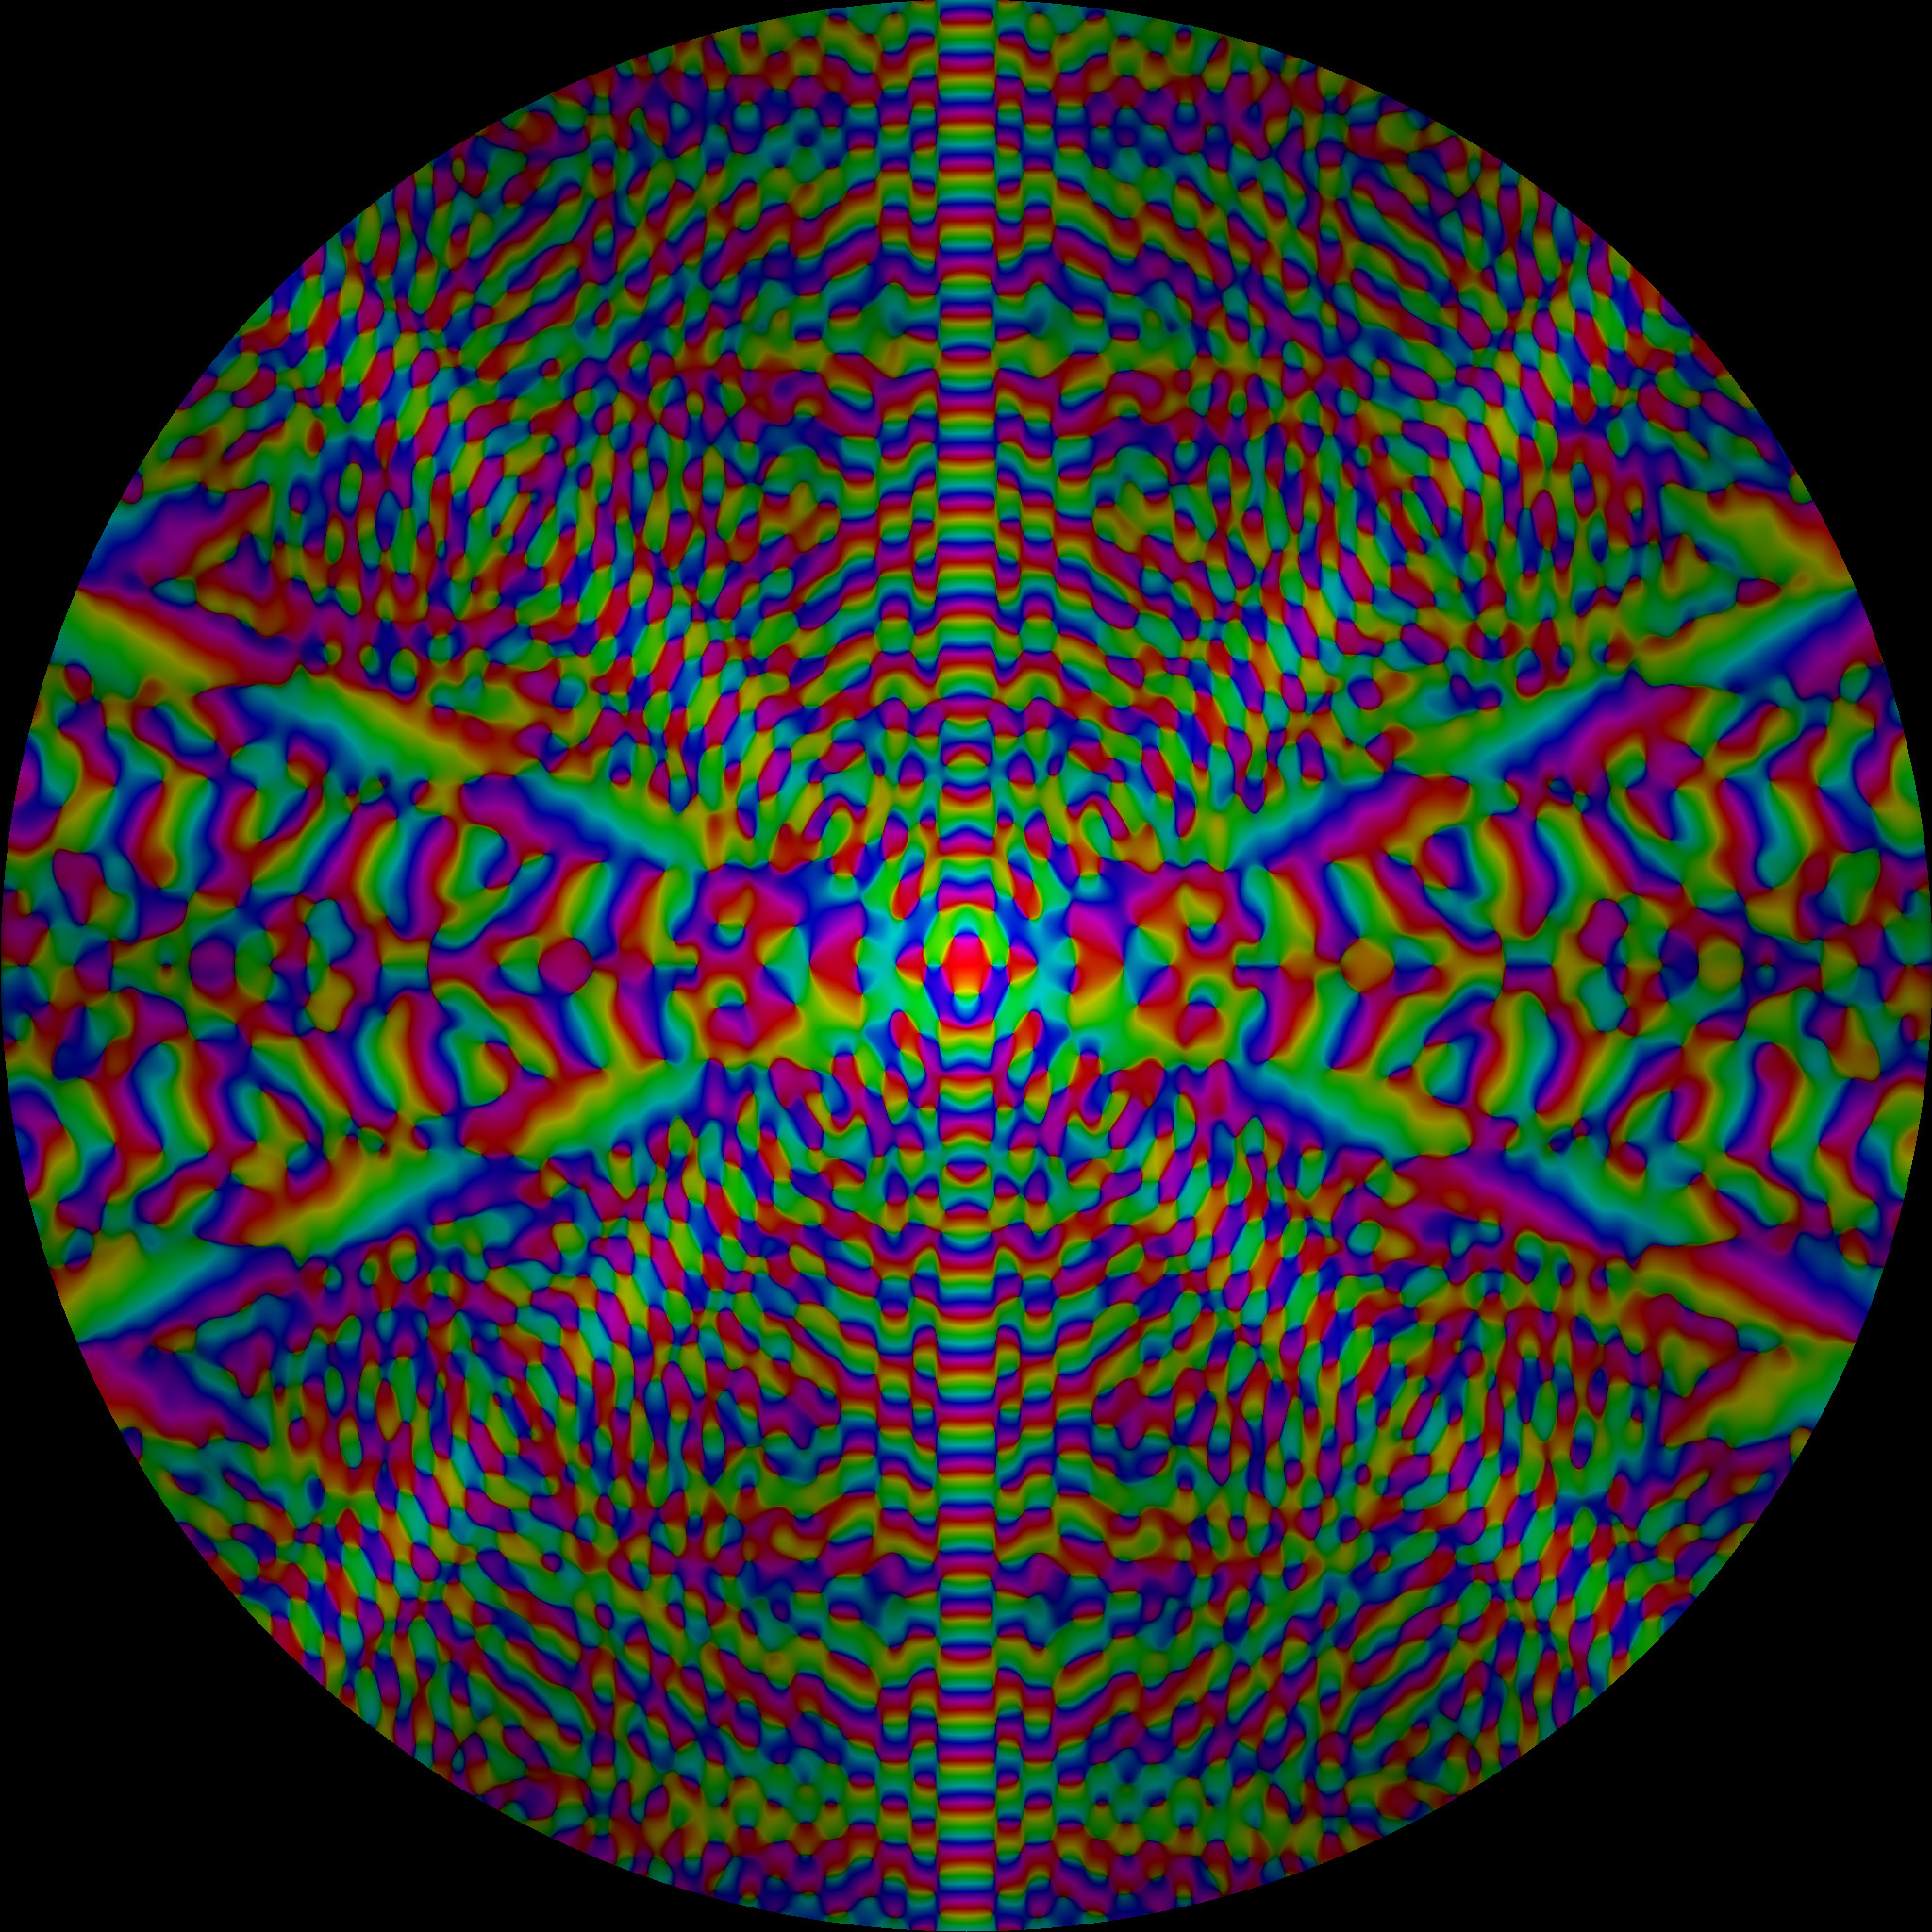
\includegraphics[width=6cm]{mathman2-backward-FT-masked.jpg}};
	\end{scope}

	\fill[color=polarcolor!10!white,opacity=0.7]
		(0,0) -- (1.5,0) arc (0:\w:1.5) -- cycle;
	\draw[color=polarcolor] (1.5,0) arc (0:\w:1.5);
	\node[color=polarcolor] at ({\w/2}:1) {$\varphi$};

	\draw[color=pointcolor,line width=1.2pt] ({\w+180}:3) -- ({\w}:3);
	\fill[color=pointcolor] (\w:\r) circle[radius=0.08];
	\node[color=pointcolor] at (\w:\r) [above left] {$(r,\varphi)$};

	\begin{scope}[rotate=\w]
	\clip (0,0) circle[radius=3.08];
	\foreach \d in {-5,-4.5,...,5}{
		\fill[color=pointcolor] (\d,0) circle[radius=0.05];
	}
	\end{scope}

	\draw[->,color=polarcolor,line width=1.2pt]
		(0,0) -- (3.3,0) coordinate[label={$r$}];
	\fill[color=polarcolor] (0,0) circle[radius=0.05];
\end{scope}

\node at (3.8,0.7) [above] {$\mathscr{F}$};
\draw[->] (3.1,0.7) -- (4.5,0.7);
\node at (3.8,-0.7) [below] {$\mathscr{F}^{-1}$};
\draw[<-] (3.1,-0.7) -- (4.5,-0.7);

\node at (3.8,-6.9) [above] {$\mathscr{F}_r$};
\draw[->] (3.1,-6.9) -- (4.5,-6.9);
\node at (3.8,-8.3) [below] {$\mathscr{F}_r^{-1}$};
\draw[->] (4.5,-8.3) -- (3.1,-8.3);

\node at (0.7,-3.8) [right] {$\mathscr{R}$};
\draw[->] (0.7,-3.1) -- (0.7,-4.5);
\node at (-0.7,-3.8) [left] {$\mathscr{R}^{-1}$};
\draw[->] (-0.7,-4.5) -- (-0.7,-3.1);

\draw[->] (6.3,-3.1) -- (6.3,-4.5);
\draw[->] (8.9,-4.5) -- (8.9,-3.1);
%\fill[color=white,opacity=0.7] (6.0,-4.0) rectangle (9.1,-3.6);
\node at (7.6,-3.8) {Polarkoordinaten};

\end{tikzpicture}
\end{document}

